\documentclass[11pt, twoside, a4paper]{book}

\usepackage{graphicx}
\usepackage[utf8]{inputenc}
\usepackage{ngerman}
%\usepackage{lineno}
\usepackage{verbatim}
\usepackage[squaren]{SIunits}
\usepackage{amsmath}
\usepackage{amsfonts}
\usepackage{amssymb}
\usepackage{enumitem}
\usepackage{fancyhdr}
\usepackage{textcomp}
\usepackage{subcaption}
\usepackage[noadjust]{marginnote}
\usepackage{tikz}
\usepackage{nicefrac}
\usepackage{framed}
\usepackage{import}

\usetikzlibrary{calc,intersections}
\usetikzlibrary{arrows}
\usetikzlibrary{decorations.markings}
\usetikzlibrary{decorations.pathreplacing}
\usepackage[european resistors]{circuitikz}
\usepackage[ 
    top=2cm, 
    bottom=2cm, 
    outer=3cm, 
    inner=3cm,
    marginparwidth=2.5cm,
		headheight=14pt
  ]{geometry}

\usepackage{parskip}
\usepackage{pdfpages}

\setlength{\parindent}{0pt}

\newcommand{\experimentheader}[4]
{
  \iftutor{{\bf Schwierigkeitsgrad:} #1\\}
  \iftutor{{\bf Dauer:} #2\\}
  {\bf Ger\"ate:} #3\\
  {\bf Bauteile:} #4
}

\newcommand{\hintboxNone}{0}
\newcommand{\hintboxExclamation}{1}
\newenvironment{hintbox}[4][\hsize]
{
  \def\FrameCommand
  {%
    {\color{#3}\vrule width 3pt}%
    \hspace{0pt}%must no space.
    \fboxsep=\FrameSep\colorbox{#4}%
  }%
  \MakeFramed{\hsize#1\advance\hsize-\width\FrameRestore}%
  \mbox{\textbf{#2}:}%
}
{
  \endMakeFramed
}
\newcommand{\xhintbox}[3]
{
  \begin{hintbox}{Achtung}{red!50}{red!10}
    #3
  \end{hintbox}
}

\newenvironment{hint}
{
  \begin{hintbox}{Hinweis}{green!50}{green!10}
}
{
  \end{hintbox}
}

\newenvironment{definition}
{
  \begin{hintbox}{Definition\\}{white!50}{white!10}
}
{
  \end{hintbox}
}

\newenvironment{important}
{
  \begin{hintbox}{Hinweis}{gray!50}{gray!10}
}
{
  \end{hintbox}
}

\newenvironment{jason}
{
  \begin{hintbox}{Achtung}{red!50}{red!10}
}
{
  \end{hintbox}
}

\newcommand{\mandatoryenumi}
{
  \renewcommand{\labelenumi}{\arabic{enumi}.} 
}
\newcommand{\optionalenumi}
{
  \renewcommand{\labelenumi}{$\bigstar$\quad\arabic{enumi}.} 
}
\newcommand{\mandatoryenumii}
{
  \renewcommand{\labelenumii}{(\alph{enumii})} 
}
\newcommand{\optionalenumii}
{
  \renewcommand{\labelenumii}{$\bigstar$\quad(\alph{enumii})} 
}
\newcommand{\icname}[1]{\mbox{\tt #1}}


  %\newcommand{\iftutor}[1]{}
\newcommand{\ifnotutor}[1]{#1}

  \newcommand{\iftutor}[1]{#1}
\newcommand{\ifnotutor}[1]{}


\newenvironment{tutorhint}{\comment}{\endcomment}
\newenvironment{todo}{\comment}{\endcomment}
\newenvironment{solution}{\comment}{\endcomment}
\iftutor
{
  \renewenvironment{todo}
  {
    \hintbox{Todo}{red!50!yellow!90}{red!50!yellow!20}
  }
  {
    \endhintbox
  }
  \renewenvironment{tutorhint}
  {
    \hintbox{Tutorenhinweis der Stunde}{blue!50}{blue!10}
  }
  {
    \endhintbox
  }
  \renewenvironment{solution}
  {
    \hintbox{L\"osung}{black!80}{black!5}
  }
  {
    \endhintbox
  }
}
\newcommand{\etutorhint}[1]
{
  \iftutor{
    \tutorhint
      #1
    \endtutorhint
  }
}
\newcommand{\esolution}[1]
{
  \iftutor
  {
    \solution
    #1
    \endsolution
  }
}
\newcommand{\etodo}[1]
{
  \iftutor
  {
    \todo
    #1
    \endtodo
  }
}



\begin{document}

\renewcommand{\thechapter}{\arabic{chapter}}
\setcounter{chapter}{11}
\def\chaptername{Versuch}

\chapter{Kennlinien verschiedener Leiter}
\label{v:12}

Die Kennlinie eines Leiter gibt an, wieviel Strom f"ur eine bestimmte angelegte Spannung durch diesen Leiter flie{\ss}t. In diesem Versuch werden Sie die Kennlinien einiger der meistgenutzten Leiter vermessen.

%------------------------------------------------
\section{Stichworte}
%------------------------------------------------

Spannung und Strom; Widerstand; Ohm'sche Gesetze; Temperaturabh"angigkeit von Widerst"anden; Leiter, Halbleiter und Isolatoren.

%------------------------------------------------
\section{Literatur}
%------------------------------------------------

Gehrtsen, Kapitel 6.1.2, 6.3.1 - 6.3.4, 6.4.3, 14.3.4, 14.4.1

%------------------------------------------------
\section{Anwendungsbeispiele}
%------------------------------------------------

So ähnlich wie das Thermoelement aus dem vorherigen Versuch werden temperaturempfindliche Widerstände zur schnellen Messung von Temperaturen benutzt. Einer der Vorteile gegenüber dem Thermoelement ist, dass diese auch als \textit{Widerstandsthermometer} bezeichneten Meßgeräte keine konstante Vergleichstemperatur brauchen.\\
Man kann hierzu Widerstände benutzen, bei denen der Widerstand mit der Temperatur steigt (\textit{Kaltleiter}, \textit{PTC}) oder fällt (\textit{Heißleiter, NTC})

%------------------------------------------------
\section{Theoretischer Hintergrund}
%------------------------------------------------

\subsection{Elektrischer Widerstand und das Ohm'sche Gesetz}

Bei allen Leitern gibt es einen Zusammenhang zwischen der Spannung $U$, die an den beiden Polen des Leiters angelegt wird, und der Stromst"arke $I$ des durch den Leiter flie{\ss}enden Stroms.
\begin{equation}\label{eq:Ohm}
U = R\cdot I \; .
\end{equation}
Den Proportionalit"atsfaktor $R$ nennt man den (ohmschen) \textit{Widerstand} des Leiters. \\
Ausser dem rein ohmschen Widerstand gibt es noch weitere Faktoren, zusammengefasst unter dem Begriff \textit{Impedanz}, die die Kennlinie $I=f(U)$ des Leiters beeinflussen. Diese wollen wir hier allerdings au{\ss}er Acht lassen (auch wenn ihre Behandlung sehr "ahnlich zu den ohmschen Widerst"anden ist).

\noindent
Bei einem homogenen ohmschen Material (Z. Bsp. ein St"uck Kupferdraht) ist der Widerstand $R$ proportional zur L"ange $l$ und umgekehrt proportional zum Querschnitt $A$ des Leiters:
\begin{equation}
R = \frac{\rho l}{A} \; .
\end{equation}
$\rho$ hei{\ss}t \textit{spezifischer Widerstand} des Materials.\\
Metalle leiten um so schlechter, je hei{\ss}er sie sind, bei Halbleitern ist es umgekehrt. F"ur kleinere Temperaturbereiche kann man eine lineare Temperaturbh"angigkeit des spezifischen Widerstandes annehmen:
\begin{equation}
\rho = \rho_0(1+\alpha T)\; .
\end{equation}
$\alpha$ hei{\ss}t Temperaturkoeffizient des Widerstandes. Er ist positiv f"ur Metalle (PTC- oder Kaltleiter) und negativ f"ur Halbleiter (NTC- oder Hei{\ss}leiter).

\subsection{Energie und Leistung elektrischer Str"ome}

Wenn sich eine Ladung $Q$ zwischen zwei Orten verschiebt, zwischen denen die Spannung $U$ herrscht, wenn sie also im Potenzial um $U$ absinkt, wird die Energie
 \begin{equation}
  W = Q\cdot U
 \end{equation}
frei. In Leitern geht diese Arbeit in die W"armeenergie des Leiters oder seiner Umgebung "uber. Die Leistung, welche den Leiter erhitzt, ergibt sich aus der Definition des Stroms:
 \begin{equation} \label{eq:Joule}
  P = \dot{W} = U\cdot\dot{Q} = U\cdot I \; .
 \end{equation}
Diesen Zusammenhang nennt man das \textit{Gesetz von Joule}.\\
F"ur einen ohmschen Leiter kann man, mit Gleichung \ref{eq:Ohm}, die Leistung auch schreiben als:
 \begin{equation}
  P = UI = I^2 R= \frac{U^2}{R}\; .
 \end{equation}

\subsection{Halbleiter, B"andermodell, etc.}

Wenn sich Atome in einem Kristallgitter befinden, nehmen sie einen sehr kleinen Abstand (wenige \AA) zueinander ein. Dann k"onnen die Elektronen "uber viele Atomabst"ande hinweg miteinander wechselwirken. Dies f"uhrt zu einer Aufweitung der (im Einzelatom noch als diskrete Niveaus vorliegenden) möglichen Energiewerte zu ausgedehnten Energiebereichen, den sogenannten Energiebändern. Da die Energiebänder je nach Aufweitung und Atomart verschieden zueinander liegen, können Bänder sich überlappen oder durch Energiebereiche, in der nach der Quantenmechanik keine erlaubten Zustände existieren (Energie- oder Bandlücke), getrennt sein. Das h"ochste besetzte Band wird \textit{Valenzband} genannt, das n"achsth"ohere Band hei{\ss}t \textit{Leitungsband}.\\
Die Fermienergie ist ein physikalischer Begriff aus der Quantenstatistik. Sie gibt die höchste Energie an, die ein Teilchen in einem Vielteilchensystem gleichartiger Fermionen (sog. Fermi-Gas) haben kann, wenn das System als Ganzes in seinem Grundzustand ist. Alle Zustände mit Energien zwischen dem tiefstmöglichen Niveau und der Fermi-Energie sind dann mit Teilchen voll besetzt, darüber keiner. Damit liegt das Ferminiveau also genau in der Bandl"ucke von Halbleitern.\\
Bei Halbleitern ist die Bandl"ucke relativ klein (Ge: $\approx 0,7$\,eV, Si: $\approx 1,1$\,eV, GaAs: $\approx 1,4$\,eV, Diamant: $\approx 5,4$\,eV). Daraus folgt, dass eine nicht zu vernachl"assigende Wahrscheinlichkeit besteht, durch thermische Anregung Elektronen ins Leitungsband anzuregen. Diese Wahrscheinlichkeit ist nat"urlich proportional zur Temperatur, d.h. f"ur h"ohere Temperaturen wird die Leitf"ahigkeit von Halbleitern besser, daher geh"oren sie zu den Hei{\ss}leitern.

\noindent
%Die relative Lage des h"ochsten besetzten Energiebandes (Valenzband) zum n"achsth"oheren Band (Leitungsband), in welchem sich die Elektronen frei durch den Festk"orper bewegen k"onnen, kann man benutzen, um Klassen von Materialien zu unterscheiden. \\
%Bei Leitern (z. Bsp. Metalle) "uberlappen das Valenzband und das Leitungsband, so dass sehr wenig Energie ben"otigt wird, um Elektronen vom Valenz- ins Leitungsband zu heben. Thermische Anregung (die kinetische Energie der Elektronen folgt der Maxwell-Verteilung) allein f"uhrt zu einer gro{\ss}en Anzahl beweglicher Elektronen.\\
%Bei Isolatoren ist die Bandl"ucke so gro{\ss} ($E_g > 4$\, eV), dass die Anzahl der Elektronen, die thermisch ins Leitungsband angeregt werden k"onnen, vernachl"assigbar ist, d.h. es gibt im wesentlichen keine beweglichen Elektronen im Festk"orper.\\
%Bei Halbleitern ist die Bandl"ucke relativ klein (Ge: $\approx 0,7$\,eV, Si: $\approx 1,1$\,eV, GaAs: $\approx 1,4$\,eV, Diamant: $\approx 5,4$\,eV).

%------------------------------------------------
\section{Fragen zur Vorbereitung}
%------------------------------------------------

\begin{enumerate}
 %
 %\item Was soll heute im Praktikum gemessen werden? Warum?
 %%
 \item Wie sind Strom und Spannung definiert? (Erkl"aren Sie: $U_{12} = - \int_{1}^{2}{\vec{E}d\vec{r}}$)
 %
 \item Wie ist der elektrische (ohmsche) Widerstand definiert?
 %
 \item Wie h"angt der elektrische Widerstand von den r"aumlichen Dimensionen des Leiters und vom Material ab?
 %
 \item Was mi{\ss}t ein Ampere-/Voltmeter? Wie wird es in den Stromkreis geschaltet?
 %
 %\item Erkl"aren Sie das B"andermodell eines Halbleiters. (Definition: Valenzband, Leitungsband, Ferminiveau)\\
 % Warum kann ein volles Band keinen Strom leiten?
 %
 \item Wie sieht die Bandstruktur eines Isolators, Halbleiters und Leiters aus? Skizze.
 %
 \item Erl"autern Sie die Temperaturabh"angigkeit des spezifischen Widerstandes $\rho$.
 %
 \item Warum (und wie) verändert sich der Widerstand eines Leiters (Metall) bei Veränderung der Temperatur? Was bedeuten PTC und NTC?
 %
 \item Warum ist das Verhalten von Halbleitern bei Temperaturveränderung entgegengesetzt dem von Leitern ? Erklärung mit Bändermodell.
 %
 \item Wie funktioniert eine Spannungsteilerschaltung?
 %
\end{enumerate}

%------------------------------------------------
\section{Durchführung} 
%------------------------------------------------

\begin{enumerate}
 %
 \item Messen Sie f"ur die Metallfadenlampe die Stromst"arke $I$ als Funktion der angelegten Spannung $U$.\\
  Fahren Sie dazu die Spannung $U$ in Schritten von 1\,V von 0\,V bis 12\,V hoch und lesen Sie die Stromst"arke $I(U)$ ab.\\
  In diesem Versuchsteil wird das Thermoelement nicht angeschlossen.
\end{enumerate}
Benutzen Sie zur Messung der Kennlinien die folgende Schaltung:
\begin{figure}[h]
	\centering
		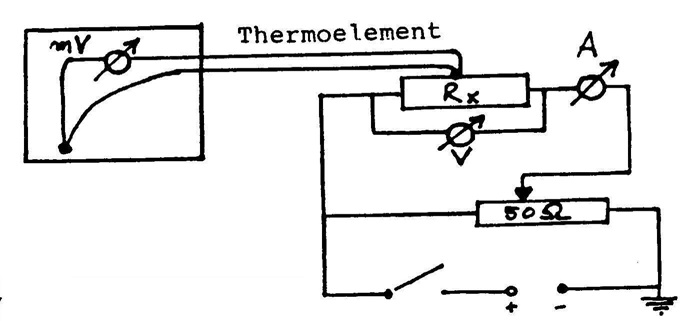
\includegraphics[width=.5\textwidth]{Versuch_11-12/Abbildungen/Schaltplan-12.jpg}
	\label{fig:Schaltplan-12}
\end{figure}

\begin{enumerate} \setcounter{enumi}{1}
 %
 \item Die NTC und PTC Widerst"ande erw"armen sich signifikant, wenn Strom durch sie flie{\ss}t. Schliessen Sie daher f"ur die Messung ihrer Kennlinien das Thermoelement direkt an die schwarzen Buchsen an. Das Thermoelement darf nicht mit dem restlichen Stromkreis verbunden sein.
 %
 \item Messen Sie f"ur den NTC und den PTC den Widerstand als Funktion der Temperatur des Bauteils.\\
  Warten Sie nach jeder Einstellungs"anderung, bis sich der Strom $I$ bei eingestellter Spannung $U$ nicht mehr "andert (ca. 1 min). Lesen Sie erst dann Strom, Spannung und Thermospannung ab.
  \begin{itemize}
   %
   \item Stellen Sie f"ur den PTC Spannungen von 0-12\,V in 1\,V-Schritten ein.
   %
   \item F"ur den NTC ver"andern Sie die Stromst"arke: Beginnen Sie bei einer hohen Stromst"arke von 300\,mA und gehen Sie in 30\,mA-Schritten herunter bis 0\,mA.
   
    \noindent
    \textbf{Achtung:} Achten Sie darauf, dass durch den NTC nie mehr als 300\,mA flie{\ss}en!\\
    Drehen Sie dazu den Strom zun"achst voll auf. Ab ca. 150\,mA steigt die Stromst"arke sehr schnell an. Regeln Sie dann den Strom entsprechend runter. Beobachten Sie die Messger"ate w"ahrend dieses Vorganges sehr genau!\\
    Lassen Sie den NTC bei eingestelltem Strom ins thermische Gleichgewicht zur"uckkehren, bevor Sie ihre Messung starten.
   %
  \end{itemize}
 %
 \item Messen Sie die Raumtemperatur.
 %
\end{enumerate}

%------------------------------------------------
\section{Auswertung} 
%------------------------------------------------

\begin{enumerate}
 %
 \item Stellen Sie die Kennlinie der Metallfadenlampe, $I=f(U)$, grafisch dar.
 %
 \item Grafische Darstellung des Widerstandes des NTC- und des PTC-Leiters als Funktion der Temperatur.
  \begin{itemize}
   \item Berechnen Sie aus der Thermospannung die Temperatur wie folgt.\\
    Im Idealfall betr"agt die Thermospannung bei Raumtemperatur 0\,V. Wenn dem nicht so ist, ziehen Sie von ihren Messwerten die bei Raumtemperatur gemessenen Thermospannung $U_{th}(RT)$ ab. Die Eichung des Thermoelementes betr"agt $a = 54\,\mu V / ^{\circ}C$. Damit errechnet sich die Temperatur in $^{\circ}C$ zu:
    \begin{equation}
     T = \frac{U_{th}(T) - U_{th}(RT)}{a} + RT
    \end{equation}
   %
   \item Berechnen Sie aus den U und I Wertepaaren den Widerstand des Leiters.
   %
   \item Tragen Sie f"ur den NTC-Leiter den nat"urlichen Logarithmus des Widerstandes $\ln(R)$ als Funktion von $1/T$ auf. Benutzen Sie die Temperatur in Kelvin.\\
    Da die Temperaturabh"angigkeit eines Hei{\ss}leiters einem Exponentialgesetz folgt:
    \begin{equation}
     R(T) = A\cdot \exp\left(\frac{\Delta E}{2k_b T}\right)
    \end{equation}
    ergibt diese Auftragung eine Gerade. Die Konstante $A$ h"angt von Bauform und Material des Hei{\ss}leiters ab.\\
    Berechnen Sie aus der Steigung der Geraden die Energiel"ucke $\Delta E$ zwischen Valenz- und Leitungsband des Halbleitermaterials, aus dem der Hei{\ss}leiter aufgebaut ist. Berechnen Sie den Fehler von $\Delta E$ aus der bekannten Fehlerfortpflanzung.
    
    \noindent
    Hinweis: $k_b = 8,62 \times 10^{-5}$\, eV/K
  \end{itemize}
 %
 \item Vergleichen Sie die gemessene Energiel"ucke mit Literaturwerten und diskutieren Sie die Fehlerquellen in Ihrer Messung.
 %
\end{enumerate}

\end{document}